\documentclass[12pt]{amsart}
%\pagestyle{empty} 
\setlength{\topmargin}{-0.4in} % usually -0.25in
\addtolength{\textheight}{1.5in} % usually 1.25in
\addtolength{\oddsidemargin}{-0.8in}
\addtolength{\evensidemargin}{-0.8in}
\addtolength{\textwidth}{1.5in} %\setlength{\parindent}{0pt}

% macros
\usepackage{wrapfig,caption,palatino,tabularx}
\usepackage{amssymb,xspace}
\usepackage[final]{graphicx}
\usepackage{tikz}
\usepackage[colorlinks=true]{hyperref}

\newcommand{\regfigure}[3]{\includegraphics[height=#2in,width=#3in]{#1.eps}}

\newtheorem*{lem*}{Lemma}

\newcommand{\mtt}{\texttt}
\newcommand{\mtl}[1]{{\texttt{>>#1}}}
\usepackage{alltt}
\usepackage{verbatim} % for "comment" environment
\newcommand{\mfile}[1]
{\medskip\begin{quote} \begin{alltt}\input{C:/MATLABR11/work/#1.m}\end{alltt} \end{quote}\medskip}

\newcommand{\CC}{{\mathbb{C}}}
\newcommand{\RR}{{\mathbb{R}}}
\newcommand{\eps}{\epsilon}
\newcommand{\ZZ}{{\mathbb{Z}}}
\newcommand{\ZZn}{{\mathbb{Z}}_n}
\newcommand{\NN}{{\mathbb{N}}}
\newcommand{\bu}{\mathbf{u}}
\newcommand{\bv}{\mathbf{v}}
\newcommand{\ip}[2]{\mathrm{\left<#1,#2\right>}}
\newcommand{\erf}{\operatorname{erf}}
\newcommand{\spn}{\operatorname{span}}

\newcommand{\Matlab}{\textsc{Matlab}\xspace}
\newcommand{\Octave}{\textsc{Octave}\xspace}
\newcommand{\pylab}{\textsc{pylab}\xspace}
\newcommand{\MOP}{\textsc{Matlab}\big|\textsc{Octave}\big|\textsc{pylab}\xspace}

\newcommand{\prob}[1]{\bigskip\bigskip\noindent\large\textbf{#1.} \normalsize}
\newcommand{\bookprob}[1]{\bigskip\bigskip\noindent\large\textbf{Exercise #1.} \normalsize}
\newcommand{\ppart}[1]{\medskip\noindent\large\textbf{\emph{#1})}\normalsize}

\begin{document}

\begin{center}
\LARGE Math 615 Numerical Analysis of \\ Differential Equations

\large \medskip
Spring 2023, UAF
\end{center}

\thispagestyle{empty}
\bigskip

\noindent \emph{instructor:} \begin{minipage}[t]{0.5\textwidth} Ed Bueler \\ \texttt{elbueler\@@alaska.edu} \end{minipage} \hfill \emph{CRN:}\, \begin{minipage}[t]{0.25\textwidth} 34643 (in-person) \\ 36848 (sync zoom) \end{minipage}

\medskip
\noindent \emph{course website:} \href{https://bueler.github.io/nade/}{\texttt{bueler.github.io/nade/}} \hfill \emph{room \& time:} \begin{minipage}[t]{0.25\textwidth} Brooks 302 \\ MWF 10:30--11:30 am \end{minipage}

\bigskip
\noindent \emph{textbook:} \begin{minipage}[t]{0.6\textwidth} R.~J.~LeVeque, \emph{Finite Difference Methods for Ordinary and Partial Differential Equations}, SIAM Press 2007 {\footnotesize (ISBN-13: 978-0-898716-29-0)} \end{minipage}

\bigskip
\noindent \emph{practical prerequisites:} Linear algebra, some analysis or differential equations, some computer programming, and graduate standing or permission of instructor.

\smallskip
\noindent (\emph{officially:} CS 201, Math 314, Math 426, Math 432)

%\vspace{-16mm}
%\hfill 
\includegraphics[height=38mm]{../../images/GitHub-Mark-32px.png}
%\vspace{5mm}

\begin{wrapfigure}{l}{0.3\textwidth}
  %\centering
    %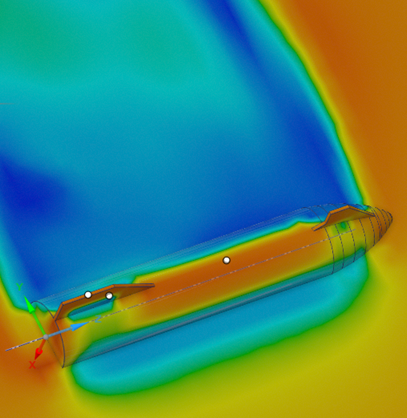
\includegraphics[width=0.4\textwidth]{../../images/Starship-simul-3.png}
\begin{tikzpicture}[scale=3.5]
  \draw[->,gray,very thin] (0.0,0.0) -- (1.2,0.0) node[below] {$x$};
  \draw[->,gray,very thin] (0.0,0.0) -- (0.0,1.2) node[left] {$y$};
  \draw[line width=1.0pt] (0.0,0.0) -- (0.0,1.0) -- (1.0,1.0) -- (1.0,0.0) -- cycle;
  \node at (0.75,-0.1) {$i$};
  \node at (-0.1,0.666667) {$j$};
  \filldraw (0.50,0.666667) circle (0.8pt);
  \filldraw (0.75,0.666667) circle (0.8pt);
  \filldraw (1.00,0.666667) circle (0.8pt);
  \filldraw (0.75,0.5) circle (0.8pt);
  \filldraw (0.75,0.833333) circle (0.8pt);
  \draw[line width=2.0pt] (0.50,0.666667) -- (1.00,0.666667);
  \draw[line width=2.0pt] (0.75,0.5)  -- (0.75,0.833333);
  \draw[xstep=0.25,ystep=0.166667,black,thin] (0.0,0.0) grid (1.0,1.0);
\end{tikzpicture}
\end{wrapfigure}

\bigskip
Numerical approximations of partial differential equations (PDEs) and ordinary differential equations (ODEs) generate simulations of fluid flow, electromagnetic fields, thermodynamics, elastic deformation, quantum mechanics, chemistry, and finance.  This course emphasizes finite difference methods for PDEs, with mathematical understanding of stability and convergence, but it also covers ODE numerical schemes.

\smallskip
Every homework includes numerical experimentation using Matlab, Python, Julia, or your preferred language.  There is a student-chosen project and two
in-class exams.

\smallskip
At the end of the course you will be able to evaluate and use numerical tools for solving many scientific and engineering problems based on differential equations.  You will have a mathematical start on the finite element method and spectral methods.

\smallskip
While the course is delivered hybrid, in-person attendance is recommended!

\bigskip
\noindent
\begin{minipage}[t]{0.5\textwidth} \emph{Topics:}
\begin{itemize}
\item thinking with matrices and vectors
\item routine visualization
\item finite differences
\item stability and convergence
\item explicit versus implicit
\item adaptive time-stepping
\item stiffness
\item diffusion and transport
\item method of lines
\item using iterative linear algebra
\item Newton's method
\end{itemize}
%\mbox{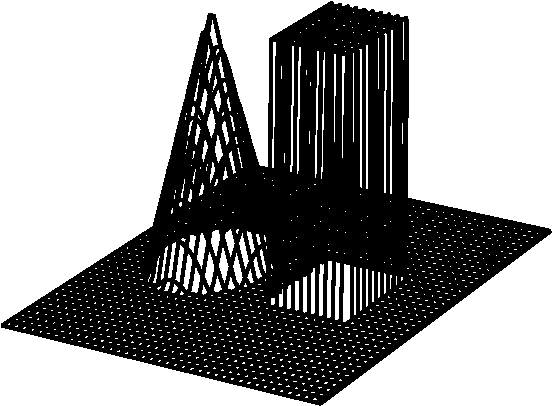
\includegraphics[width=0.45\textwidth]{../../images/rotationinitial.pdf} 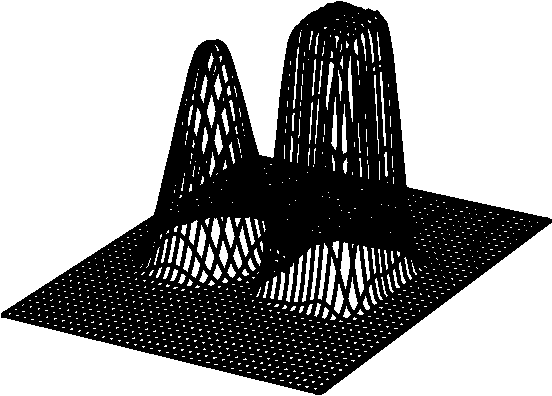
\includegraphics[width=0.45\textwidth]{../../images/rotationfinal.pdf}}
\end{minipage}
\begin{minipage}[t]{0.5\textwidth}
\phantom{foo}

\hfill 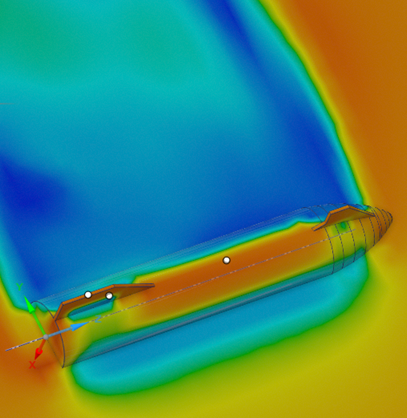
\includegraphics[width=0.75\textwidth]{../../images/Starship-simul-3.png}
\end{minipage}

%\begin{minipage}[t]{0.45\textwidth}
%\smallskip
%\centering
%
\includegraphics[height=52mm]{../../images/GitHub-Mark-32px.png}
%\end{minipage}

\end{document}

